\documentclass[12pt]{scrartcl}

\usepackage[T1]{fontenc}
\usepackage[ngerman]{babel} % Silbentrennung
\usepackage[utf8]{inputenc} % Umlaute
\usepackage{graphicx}
\usepackage[style=authortitle-icomp]{biblatex}
\usepackage[babel,german=guillemets]{csquotes}

\usepackage{float}
\usepackage{pdfpages}

\usepackage{xcolor}
\definecolor{dark-red}{rgb}{0.4,0.15,0.15}
\definecolor{dark-blue}{rgb}{0.15,0.15,0.4}
\definecolor{medium-blue}{rgb}{0,0,0.5}

\usepackage{hyperref}
\hypersetup{
    colorlinks, linkcolor={dark-red},
    citecolor={dark-blue}, urlcolor={medium-blue}
}


\begin{document}



%%%%%%%%%%%%%%%%%%%%%%%%%%%%%%%%%%%%%%%%%%%%%%%%%%%%%%%%%%%%%%%%%%%%%%%%%%%%%

% Deckblatt
% Fehlt noch WS 13/14

\begin{titlepage}

\begin{center}


\includegraphics[width=1.0\textwidth]{fhkoeln.jpg}
\\[2cm]
\textsc{\LARGE EIS}
\\[0.2cm]
{\Large Entwicklung Interaktiver Systeme}
\\[3cm]
\textsc{\Huge Konzept}

\vfill

\textsc{\Large Team}\\
Duc Duy Khuong (11084720)\\
Robert Kellermann (11082910)
\\[1cm]
\textsc{\Large Betreuer}\\
Prof. Dr. Kristian Fischer\\
Prof. Dr. Gerhard Hartmann\\
Renée Schulz\\
Christopher Messner
\\[2cm]
\today

\end{center}

\end{titlepage}

\tableofcontents

\newpage

%%%%%%%%%%%%%%%%%%%%%%%%%%%%%%%%%%%%%%%%%%%%%%%%%%%%%%%%%%%%%%%%%%%%%%%%%%%%%

\section{Einführung}

Musik spielt bei vielen Menschen im alltäglichen Leben eine wichtige Rolle. Ob man Musik hört oder selber ein Instrument spielt, ist da jedem selber überlassen. Diejenigen, die sich sich für Letzteres entscheiden, wollen dann meistens auch mit anderen Musikern zusammen Projekte starten und gründen eine Band.

Die Organisation der Band spielt dabei eine übergeordnete Rolle, denn die Bandproben hängen vom Zeit- und Ortsfaktor ab, wann hat Jeder Zeit und wo wird der Bandraum sein. Wenn diese Fragen geklärt sind, besteht die Absicht darin, die Zeit der Probe so effizient wie möglich zu nutzen.

%% vielleicht noch etwas ausführlicher?

\subsection{Problem}

Ein grundlegendes Problem ist der Umgang mit neuen Ideen. Wenn beispielsweise ein Musiker eine Idee zu einem neuen Song hat, etwa ein Riff oder eine kurze Melodie, muss er bis zur nächsten Probe warten, um sie der Band vorzustellen. Zu dieser Idee steuern die anderen Musiker dann meist ihre Ideen bei und entwickeln somit gemeinsam einen neuen Song. Dieser kreative Prozess nimmt jedoch viel Zeit in Anspruch. Aufgrund der wertvollen Zeit im Proberaum entsteht somit ein Druck auf den Bandmitgliedern und der Kreativität der Musiker wird möglicherweise kein freier Lauf gelassen.

\subsection{Idee}

Um diesen Zeitdruck beim Komponieren im Proberaum zu vermeiden, wäre es hilfreich, neue Ideen auch außerhalb der Bandproben festzuhalten und mit den Bandkollegen zu teilen. Ein Austausch von Ideen und das Beitragen von Einfällen und weiteren Ideen dazu könnte entweder alleine in Ruhe oder in Kommunikation mit den anderen Bandmitgliedern über das Internet erfolgen. Dadurch könnte die Zeit im Proberaum für das tatsächliche Proben des Zusammenspiels in der Band und den letzten Schliff an neuen Songs genutzt werden, während die kreativen, meist sehr zeitaufwändigen Kompositionsprozesse außerhalb der Proberaumatmosphäre stattfinden.

%%%%%%%%%%%%%%%%%%%%%%%%%%%%%%%%%%%%%%%%%%%%%%%%%%%%%%%%%%%%%%%%%%%%%%%%%%%%%

\section{Ziele}

In dieser Zielhierarchie soll deutlich gemacht werden, welche kurz- und langfristigen Ziele das Projekt \emph{CoMusic} ausmachen. Danach soll dann in der Zielpriorisierung aufgezählt werden, welche dieser Ziele die Besonderheiten und die Alleinstellungsmerkmale des Projektes darstellen.
% Einführung zu den Zielen vllt noch etwas ausführlicher? Zielpriorisierung besser erklären?

\subsection{Strategische Ziele}

% zu wenig Ziele definiert
% ausformulieren, detaillierter, mehr eingehen und verschärfen
\begin{itemize}


\item Der Zeitdruck, der bei kreativer Arbeit an neuen Songideen auftritt, kann vermieden werden. Der begrentze Faktor Zeit soll eine verminderte Rolle spielen
\item Aufkommende Ideen oder Einfälle sollen in Ruhe festzuhalten sein
\item Aktivitäten einer Band, die sonst während der Proben durchgeführt werden, sollen außerhalb ermöglicht werden
\end{itemize}

Langfristiges Ziel des Systems soll sein, alle beeinträchtigenden Aspekte, die beim gemeinsamen musizieren entstehen können, zu verringern. Es wird versucht die Aktivitäten auch auf außerhalb der Proben zu verlagern und zu erleichtern, damit effizienter gearbeitet werden kann.

\subsection{Taktische Ziele}


\begin{itemize}
\item gemeinsam nutzbare Plattform
\item Das Teilen und Ausarbeiten von Songideen soll in Ruhe außerhalb des Proberaumes geschehen können
\item Unabhängiges Arbeiten voneinander
\item Kommunizieren der Bandmitglieder über Ideen soll möglich sein
\
\end{itemize}

Taktisches Ziel ist die Entwicklung eines Systems, das Musikern eine gemeinsam nutzbare Plattform gibt, welche die Funktion bereitstellt gemeinsam an Kompositionen arbeiten zu können. Dabei steht nicht in Vordergrund wo und wann dies geschehen soll, sondern viel mehr, dass es überall möglich ist. Das Erstellen und Bearbeiten von Kompositionen ist unabhängig voneinander und geschieht außerhalb des Proberaumes. 
Zudem ist die Kommunikation dabei ein wichtiger Aspekt, die einzelnen Mitglieder können sich über Ideen austauschen und diese kommentieren oder ähnliches.
% Kollaborativ ist zu wolkig -> mehr spezifizieren

\subsection{Operative Ziele}

Um die strategischen und taktischen Ziele zu erfüllen werden zunächst geeignete Vorgehens- und Gestaltungsmethoden der Mensch-Computer-Interaktion ausgewählt. Darauf hin werden die technischen Anforderungen des Systems festgelegt und schließlich ein Prototyp entwickelt, welches die Funktionalitäten des System demonstriert.

\begin{itemize}
\item Vorgehensmodelle und Gestaltungsmethoden der MCI auswählen
\item Festlegung der technischen Anforderungen
\item Entwicklung eines Prototyps 
\end{itemize}

%% to add: echtzeitkommunikation, übertragene daten: änderungsinformationen, neue kommentare

\subsection[Geplante Funktionalitäten]{Geplante Funktionalitäten des Systems}

\begin{itemize}
\item Band- und Musikerverwaltung (einzelne Accounts für die Musiker, gemeinsamer Bereich für die jeweiligen Bands
\item kollaboratives Arbeiten an MIDI-Spuren innerhalb einer Kompositionsidee
\item Echtzeitaktualisierung der Spuren
\item kompositionsbezogene Kommunikation der Bandmitglieder (Chatroom, Notizen o.Ä.)
\item Optional: Generierung von Notenblättern und Tabulaturen anhand der MIDI-Dateien
\item ------------------------------
\item Band- und Musikerverwaltung
\item Zusammenarbeit an einer Kompositionsidee 
\item Ermöglichung der Echtzeit-Zusammenarbeit trotz örtlicher Unabhängigkeit
\item Option: Generierung von Musikblättern mit einheitlicher Musiknotation
\end{itemize}


%% SCHWERPUNKT auf echtzeitkollaboration !!!



% geplante Funktionalitäten: zu technisch
% Zielpriorisierung textuell formulieren, zu ungenau
% zu ungenau: Begründung warum MIDI

%% Hier evtl zusammenfassung als tabelle

%%%%%%%%%%%%%%%%%%%%%%%%%%%%%%%%%%%%%%%%%%%%%%%%%%%%%%%%%%%%%%%%%%%%%%%%%%%%%

\section{Mensch-Computer-Interaktion}

% zu allgemein, nicht projektbezogen, besser darlegen
% Stakeholderanalyse noch spezifischer, Grundlage für Begründungen
% wirkt vorgegriffen/zusammengewürfelt

\subsection{Abwägung Nutzerzentrierte/Nutzungszentrierte Gestaltung}
Um eine geeignete Grundlage zu schaffen, damit eine erfolgreiche Umsetzung des System erfolgen kann, sollte eine vollständige und durchdachte Planung stattfinden. Dazu zählt die Konzeptionierung, Evaluation, Gestaltung und die Entwicklung. 
Mit Hilfe verschiedener Vorgehensmodelle und Methoden der Mensch-Computer-Interaktion ist es möglich dies zu realisieren.

Erste zentrale Frage ist es, festzustellen welche der beiden Möglichkeiten, benutzerzentrierte oder benutzungszentrierte Gestaltung, bei der Entwicklung des Systems sinnvoller ist.

Aus der Problematik bzw. der Motivation, lässt sich ableiten, dass die Entwicklung der Anwendung der Intention dient, dass die Bedüfnisse der Benutzer also die “user needs” erfüllt werden und daraus folgend eine gute “user experience” zu erreichen. 
In dem Fall sind die Benutzer, die im Hauptfokus des Projekts stehen, die Musiker, speziell die in Gruppen wie Bands etc., was bedeutet, dass das System auf die eine Zielgruppe zugeschnitten werden muss. Auch der Nutzungskontext lässt sich daraus ableiten, wodurch sich eine benutzerzentrierte Gestaltung anbietet. Die Anforderungen der Benutzer können herauskristallisiert werden wodurch das System weitesgehend angepasst werden kann.

Dadurch sollten sie möglichst auch ohne jegliche Vorkenntnisse, bis auf die in unserem spezifischen Nutzungskontext erforderten, mit dem System interagieren können.
Um dies gewährleisten zu können ist es notwendig, die Gebrauchstauglichkeit des Systems zu maximieren, d.h. die Entwicklung und Gestaltung. Alles, was ihn in der Interaktion mit dem System beeinträchtigen könnte, sollte möglichst vermieden werden. Im Gegenteil, die Anwendung sollte den Benutzer in der Verwendung unterstützen können. Dazu zählt z.B. eine nicht zu komplexe grafische Benutzeroberfläche (GUI). Die Elemente der GUI sollten so gewählt sein, dass die Gebrauchstauglichkeit hoch ist und keine Verwirrung oder Überforderung stattfindet.

\subsection{Auswahl der MCI-Methoden}

Nach der Wahl des Vorgehensmodells, werden einige Methoden der Mensch-Computer-Interaktion ausgewählt, die Informationen liefern können, welche relevant für die Entwicklung des Systems sein können.
Diese Methoden kann man in 4 Bereiche einteilen, die sich auch im Vorgehensmodell widerspiegeln:
Die Nutzungskontextanalyse
Die Benutzermodellierung
Schnittstellendesign und die
Evaluation

\subsubsection{Nutzungskontextanalyse}

Zur Nutzungskontextanalyse gehört zunächst einmal die Festlegung der Nutzungskontexte, also wofür wird das System benötigt und in welchem Fall wird es verwendet. Dazu können Szenarien und Use Cases erstellt werden um bestimmte Kontexte untersuchen zu können. Zuvor sollte jedoch die Benutzermodellierung stattfinden, damit diese vollständig umgesetzt werden.

\subsubsection{Benutzermodellierung}

Unter die Benutzermodellierung gehört das Erstellen von User Profiles, Personae oder auch die Befragung potentieller Benutzer. 

\subsubsection{Schnittstellendesign}

Sind die Nutzungsanforderungen festgelegt, so ist der nächste Schritt die Gestaltungslösung zu entwickeln. Diese können in Form von papier-basierten Prototypen, erste digitale Mockups oder Ähnliches auftreten.

\subsubsection{Evaluation}

Als finaler Schritt, findet die Evaluation statt, d.h. es wird geprüft, ob in dieser Phase die “User Needs” zufriedenstellend erfüllt sind. Falls die Evaluation der Gestaltungslösung positiv ausfällt, kann mit der Umsetzung begonnen werden, ist dies jedoch nicht der Fall, so kann mit Hilfe Iteration, die Aspekte erneut untersucht werden, die noch zu optimieren sind.

\begin{table}[!ht]

\begin{tabular}{|p{3cm}|p{3.0cm}|p{7cm}|p{2cm}|} \hline

\textbf{Bezeichnung} & \textbf{Beziehung zum System} & \textbf{Beschreibung} & \textbf{Priorität für das Projekt}\\ \hline

Bandmusiker & Anspruch & Bandmusiker erstellen mit Hilfe des Systems Projekte, welche jeweils neue Kompositionen enthalten. Sie benutzen die Anwendung, um außerhalb der Bandproben immer noch miteinander Ideen erstellen und Musik komponieren zu können. & hoch \\ \hline

Musikproduzenten & Interesse & Können das System verwenden um mit Bands bzw. Musikern zu kollaborieren oder sie zu unterstützen bei der Komposition. & mittel \\ \hline

Plattenfirma & Interesse & Vorgesetzte von Musikern und Bands. Haben ggf. Interesse daran, das System für die eigenen Musiker zu verwenden, oder auch für die eigenen Produzenten. & gering \\ \hline

Musiksoftware- hersteller & Interesse & Haben ggf. Interesse daran, das System in ihre eigene Software zu integrieren. & gering \\ \hline

Bands, die eine Zusammenarbeit mit anderen Bands planen & Anspruch, Interesse & Genau wie einzelne Musiker in einer Band, können mehrere Bands für gemeinsame Projekte, mit Hilfe des Systems, zusammenarbeiten. & hoch \\ \hline

Musikveröffent- lichungsplattform & Interesse & Die einzelnen Ideen können abgespeichert werden und auf den Plattformen für die Öffentlichkeit präsentiert werden. & gering \\ \hline

Hersteller für technisches Zubehör (z.B. Interfaces, Instrumente) & Interesse & Sind am System interessiert, da sich durch die Verwendung hardware-technische Voraussetzungen ergeben, welche den Verkauf unterstützen können. & gering \\ \hline



\end{tabular}
\caption{Stakeholderanalyse}
\end{table}





Im weiteren Verlauf werden nun die einzelnen Schritte des Vorgehensmodells durchgegangen und die dazu passenden Methoden angewendet um eine geeignete Gestaltungslösung erstellen zu können.

%%%%%%%%%%%%%%%%%%%%%%%%%%%%%%%%%%%%%%%%%%%%%%%%%%%%%%%%%%%%%%%%%%%%%%%%%%%%%

\section{Kommunikationsablauf}

% Kommunikationsmodell abstrakter (wer mit wem, welche Inhalte, syn/asyn, welche Wege/Alternativen)
% technisch zu konkret, auf einer höheren Ebene argumentieren (Echtzeitkommunikation statt Chatroom)

%- wer mit wem
%- welche inhalte
%- paradigmen syn/asyn
%- welche wege (alternativ: peer to peer)
%BEGRÜNDEN!

Im Folgenden soll die Kommunikation im System CoMusic erläutert werden. Diese ist in \ref{fig:kommunikationsmodell} dargestellt.

\begin{figure}[H]
\centering
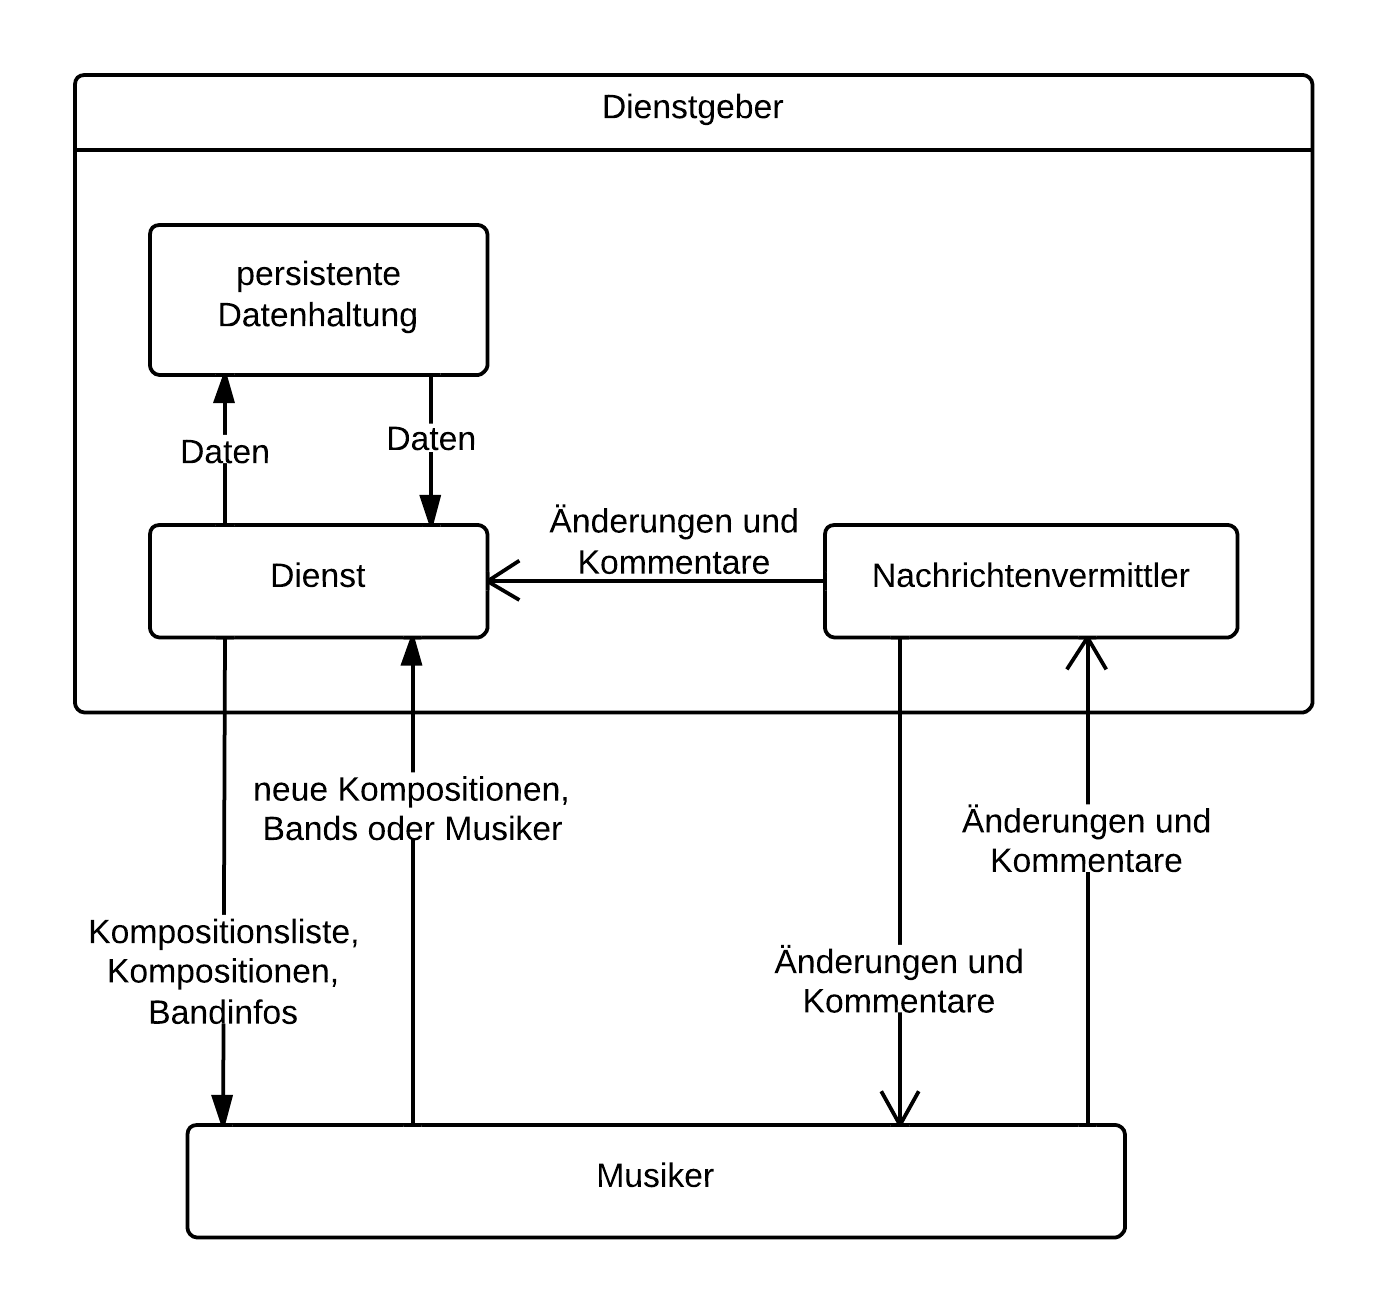
\includegraphics[scale=.25]{figures/kommunikationsmodell}
\caption{Kommunikationsmodell}
\label{fig:kommunikationsmodell}
\end{figure}

Musiker können mit dem Dienstgeber kommunizieren, um etwa neue Bands, neue Musiker oder neue Kompositionen zu erstellen. Außerdem können Sie Informationen zu ihren Bands, deren Kompositionen und bestimmte Kompositionen vom Dienst anfragen. Diese Kommunikation erfolgt nach dem synchronen Request-Response Paradigma.

Die wichtigste Kommunikation ist der Austausch von Änderungsinformationen an Kompositionen und Kommentaren in Echtzeit. Diese Informationen werden von einem Nachrichtenvermittler entgegengenommen und nach dem asynchronen Publish-Subscribe Paradigma an alle aktiven Teilnehmer gesendet. Ein weiterer Teilnehmer ist der Dienstgeber, der rein als Zuhörer fungiert und alle Änderungsinformationen in der persistenten Datenhaltung abspeichert. Eine Alternative zum Publish-Subscribe Paradigma wäre das Peer-to-Peer Paradigma, bei welchem Änderungsinformationen von einem Teilnehmer zu allen anderen aktiven Teilnehmern gesendet würden. Dieses wird hier jedoch nicht gewählt, da es viele Nachteile birgt:
\begin{itemize}
\item Alle Teilnehmer müssen sich gegenseitig kennen
\item Bei einer Änderung entsteht beim Autor je nach Anzahl der aktiven Teilnehmer viel Datenverkehr
\item Schlecht skalierbar
\end{itemize}



Um die Sicherheit der persistenten Daten zu gewährleisten, soll Kommunikationsteilnehmern des Systems in keinem Fall der direkte Zugang zur Datenhaltung ermöglicht werden. Dies erfolgt immer über den Dienstgeber, damit Anfragen und Daten validiert werden können. Die Kommunikation zwischen Dienst und der persistenten Datenhaltung erfolgt synchron, da es sich hier um Anfrage und Rückgabe beziehungsweise Modifizierung von Daten handelt.


%%%%%%%%%%%%%%%%%%%%%%%%%%%%%%%%%%%%%%%%%%%%%%%%%%%%%%%%%%%%%%%%%%%%%%%%%%%%%

\section{Systemarchitektur}

% Paradigmen kommen aus der Architektur nicht deutlich hervor, Paradigmen nicht mischen
% von Kommunikationsmodell zur Systemarchitektur führen
% Systemarchitektur konkreter, etwaige Softwarekomponenten, Logik der Komponenten (abstrakt)

% Zielplattform

% Vorgabe: java



Die Systemarchitektur, welche in Abbildung \ref{fig:systemarchitekturmodell} dargestellt ist, ist aus dem Kommunikationsmodell abgeleitet. Nachdem festgestellt wurde, wer mit wem wie kommuniziert, können nun die einzelnen, bisher eher abstrakteren Komponenten des Systems etwas genauer beschrieben werden.

\begin{figure}[H]
\centering
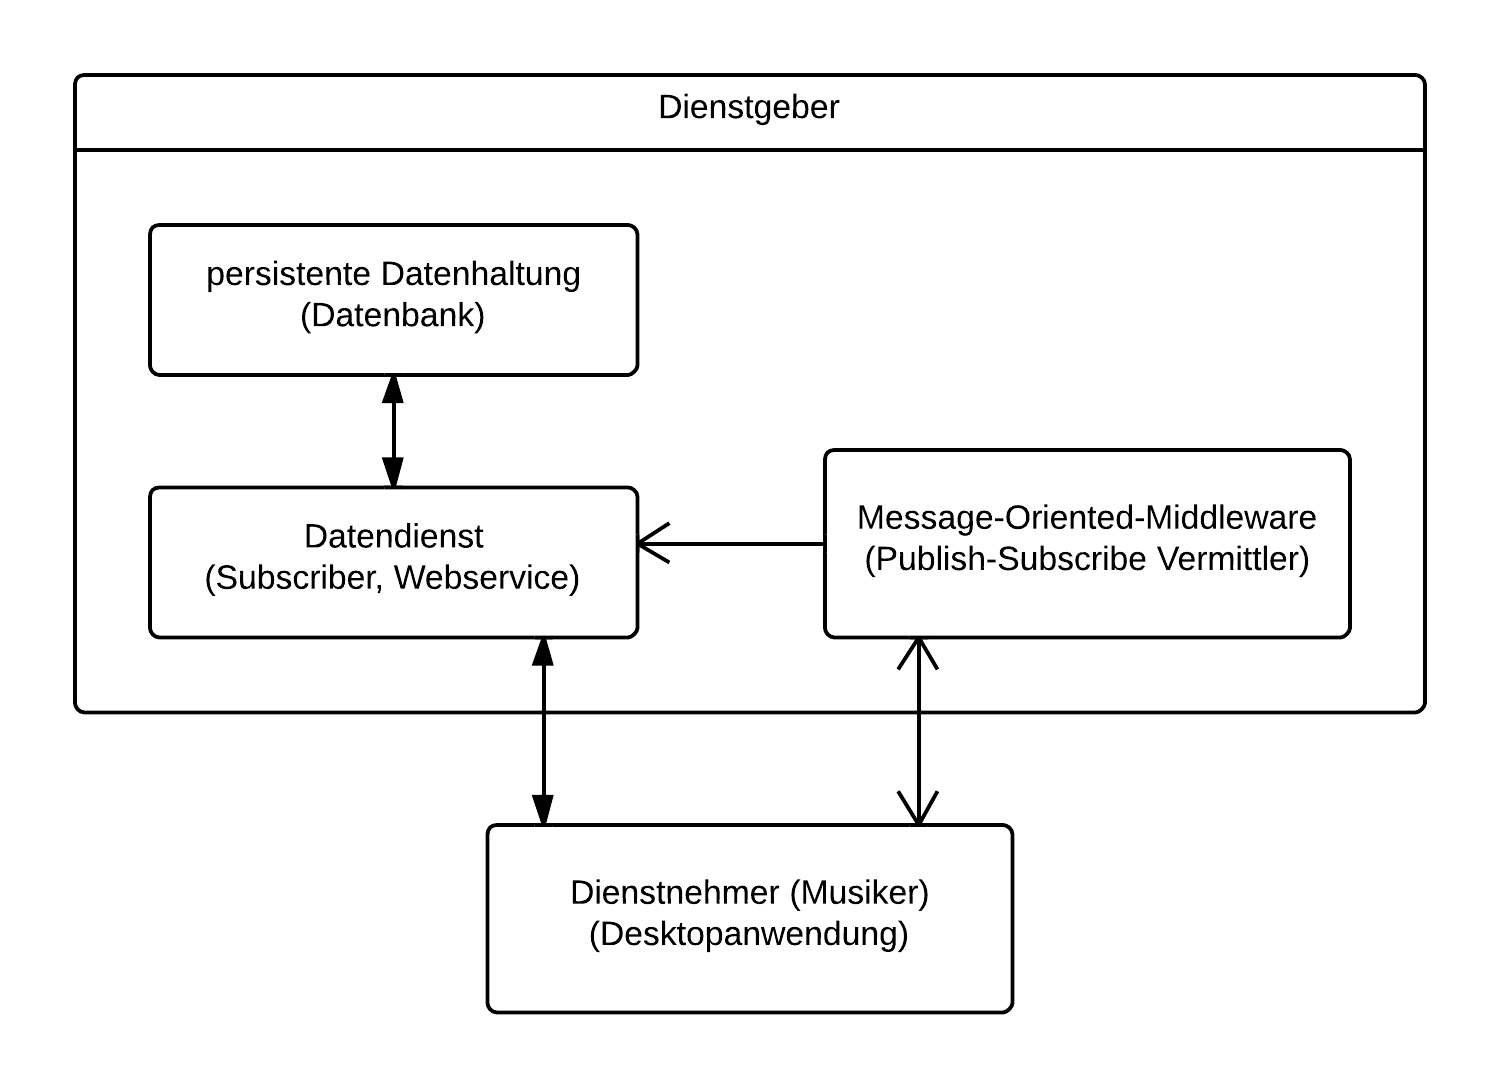
\includegraphics[scale=.25]{figures/systemarchitekturmodell}
\caption{Systemarchitekturmodell}
\label{fig:systemarchitekturmodell}
\end{figure}

\paragraph{persistente Datenhaltung}
Die persistente Datenhaltung wird aus einer Datenbank bestehen, in der alle Daten abgespeichert werden. Welche Daten hier abgespeichert werden sollen, wird im Datenmodell etwas näher erläutert.

\paragraph{Message-Oriented-Middleware}
Die MOM agiert als Vermittler in der Anwendung des Publish-Subscribe Paradigmas. Sie stellt Topics für Kompositionen zur Verfügung, auf denen Änderungen in Form von Notationsänderungen und Kommentarnachrichten in Echtzeit publiziert und an aktive Teilnehmer vermittelt wird.

\paragraph{Dienst}
Der zentrale Dienstgeber hat mehrere Aufgaben.
\begin{itemize}
\item Er fungiert als Vermittler zwischen allen Systemkomponenten und der Datenbank und validiert Anfragen und Daten.
\item Er stellt einen Webservice bereit, um Dienstnehmern das Anfragen und Modifizieren von Daten zu ermöglichen.
\item Er ist Subscriber (Zuhörer) der Message-Oriented-Middleware und erhält alle veröffentlichten Informationen, um Sie in der Datenhaltung persistent zu speichern.
\end{itemize}

Durch das direkte Speichern aller Echtzeitinformationen in der persistenten Datenhaltung erhalten alle neuen Teilnehmer immer den aktuellen Stand. Andererseits können aktive Teilnehmer jederzeit das System verlassen, ohne ungespeicherte Änderungen zu hinterlassen.

\paragraph{Dienstnehmer}
Dienstnehmer sind grafische Benutzeroberflächen in Form einer Desktopanwendung, die von den Nutzern des Systems bedient werden. Die Desktopanwendung ermöglicht den Benutzern alle nötigen Funktionen wie das Anlegen neuer Band- oder Musikerprofile und neuer Kompositionen. Ein Notationseditor in dieser Benutzeroberfläche lässt Manipulationen an Kompositionen zu, die an die MOM übermittelt werden. Ausserdem erhält der Dienstnehmer alle Manipulationen der anderen Teilnehmer und stellt sie in Echtzeit im Notationseditor dar.

%%%%%%%%%%%%%%%%%%%%%%%%%%%%%%%%%%%%%%%%%%%%%%%%%%%%%%%%%%%%%%%%%%%%%%%%%%%%%

\section{Datenmodell}
\label{sec:datenmodell}

% Datenmodell unbegründet, umstrukturieren

Das Datenmodell beschreibt, welche Daten vom System genutzt und verwaltet werden. Alle Daten, die synchron oder asynchron im System übertragen werden, werden in der zentralen, persistenten Datenhaltung gespeichert. Dies erlaubt einen zeitunabhängigen Zugriff auf alle Daten. 

\begin{description}
\item[Bandinformationen]
Informationen zu einer Band beinhalten alle notwendigen Elemente wie Bandname, zugehörige Musiker und eine Liste aller Kompositionen dieser Band. Außerdem gehört zu jeder Band ein Musiker, welcher die Rollen des Bandleiters übernimmt. Dieser kann beispielsweise derjenige sein, der die Band in das System einträgt. Diese Informationen sind für die Organisation in der Band wichtig, damit eine Zugehörigkeit zwischen Bands und Musikern vorhanden ist.
\item[Musiker]
Musiker sind die einzelnen Benutzer des Systems. Hier werden Anmeldedaten wie Benutzername und Passwort gespeichert, aber auch, zu welchen Bands er im System eingetragen ist. Musiker können in mehreren Bands gehören.
\item[Komposition]
Kompositionen bestehen zunächst aus grundlegenden Informationen wie Titel beziehungsweise Arbeitstitel, geplantes Genre und weiteren individuelle Notizen, Informationen und Anmerkungen. Weiter werden die Notationsdaten der Komposition abgespeichert. Diese bestehen aus Geschwindigkeit der Komposition und einer serialisierten Form der Notation, etwa eine Matrix mit Tonwerten.
\item[Kommentare]
Zu jeder Komposition können Kommentare und Anmerkungen gemacht werden. Diese Daten bestehen aus Datum, Autor und dem individuellen Kommentar.
\end{description}

\subsection{Datenrepräsentation}
Da die Daten in einer zentralen Datenbank gespeichert werden, übernimmt das verwendete Datenbankmanagementsystem die Aufgabe der Datenrepräsentation. Für die Übertragung der Daten zwischen den verschiedenen Systemkomponenten muss ein geeignetes Datenformat gewählt werden. Auf ein bestimmtes Format wurde sich an dieser Stelle noch nicht festgelegt.

%%%%%%%%%%%%%%%%%%%%%%%%%%%%%%%%%%%%%%%%%%%%%%%%%%%%%%%%%%%%%%%%%%%%%%%%%%%%%

\section{Abwägungen von Technologien}

\paragraph*{Synchronisieren von Daten in Echtzeit}
Für den Austausch von Kompositionsänderungen und Kommentaren in Echtzeit ist die Verwendung einer Message-Oriented-Middleware geplant. Da die Projektvorgabe Java vorgibt, bietet sich die Nutzung des Java Message Services (JMS) und eines JMS-Brokers an. Aufgrund der zweiten Vorgabe, möglichst quelloffene Software von Drittanbietern zu verwenden, fällt hier die Wahl auf den Message Broker ActiveMQ von Apache\footnote{http://activemq.apache.org/}. Dieser implementiert das JMS vollständig und bietet dadurch eine passende Lösung für das Vorhaben.

\paragraph*{Dienstnehmer}
Besonders hier schränkt die Projektvorgabe der Programmiersprache die Auswahl ein. Für die Benutzeroberfläche des Dienstnehmers wird daher Java Swing verwendet. Auch der geplante Notationseditor soll mit Swing realisiert werden.

\paragraph*{persistente Datenhaltung}
Hier wird eine relationale Datenbank ins Auge gefasst. Auf die Nutzung einer XML-Datenbank wird aufgrund ihrer nicht benötigten Komplexität und ihrer Performance im Vergleich zu relationalen Datenbanken verzichtet. Zu den wichtigsten quelloffenen Lösungen gehören in diesem Bereich MySQL und PostgreSQL. Eine Entscheidung diesbezüglich erfolgt aufgrund ausstehender Recherchen an dieser Stelle noch nicht.

\paragraph*{Musiknotation}
Musik kann in unterschiedlichen Formen notiert werden. Dies sind etwa Tabulaturen oder Noten. Da beide Notationsformen jedoch je nach Instrument verschieden Variieren (Saitenanzahl der Instrumente, Notenschlüssel etc.), bietet sich eine Notation in direkten Tonwerten und -längen an. Diese ist für Jeden unabhängig von Instrumenten nachzuvollziehen und notierbar. Hier bietet sich die Nutzung von MIDI an, da die notierten Tonwerte in MIDI Steuersignale verwandelt und in der Anwendung des Dienstnehmers abgespielt werden können. Wieder aufgrund der Projektvorgabe, müssen die Kompositionen in Java behandelt werden. Für Java gibt es im Zusammenhang mit MIDI einige verwendbare Bibliotheken. Nativ bietet Java die Bibliothek \texttt{javax.sound.midi} an. Eine etwas ausführlichere Bibliothek ist zum Beispiel JFugue\footnote{http://www.jfugue.org/}, welche eine noch einfachere Notation unterstützt. Eine Entscheidung folgt.

\paragraph*{Formate für die Datenübertragung}
Hier muss noch überlegt werden, welches Datenformat für die Übertragung verwendet wird. Möglich wären zum Beispiel XML oder JSON.

%%%%%%%%%%%%%%%%%%%%%%%%%%%%%%%%%%%%%%%%%%%%%%%%%%%%%%%%%%%%%%%%%%%%%%%%%%%%%

\section{Proof of Concepts}
Um den erfolgreichen Einsatz der verschiedenen benötigten Technologien zu gewährleisten, müssen technische Risiken minimiert und vor dem Einsatz im Projektkonzext prototypisch getestet werden. Im weiteren Projektverlauf werden vorraussichtlich die folgenden Aspekte behandelt und dazu eventuelle Alternativen im Falle von Fehlschlägen aufgezeigt.

\begin{description}
\item[Echtzeitsynchronisation]
Es soll ein einfacher Prototyp zum Senden und Empfangen von Beispielnachrichten in Echtzeit mit mehreren Dienstnehmern über den ActiveMQ Message Broker und JMS erstellt werden.
\item[Notationseditor in Swing]
Das Setzen von Tonwerten in einem grafischen Bereich und die Interaktion mit der Maus in Swing getestet werden.
\item[Datenbank]
Ein Prototyp soll Beispieldaten in einem Datenbanksystem (MySQL oder PostgreSQL) manipulieren und besonders das Abspeichern von Kompositionsspuren in einer serialisierten Notationsform testen.
\item[Synchroner Datenaustausch mit dem Dienstnehmer]
Es soll ein simpler REST Webservice implementiert werden und ein Dienstnehmer, der mit diesem Beispieldaten austauscht.
\end{description}

% fallback lösungen


%%%%%%%%%%%%%%%%%%%%%%%%%%%%%%%%%%%%%%%%%%%%%%%%%%%%%%%%%%%%%%%%%%%%%%%%%%%%%

\section{Marktrecherche und Alleinstellungsmerkmal}

%neuer Text
\subsection{kollaborative Kompositionsplattformen}
\parskip 12pt
\begin{description}
\item[Kompoz (www.kompoz.com)]
Möglichkeit der Kollaboration mit fremden Personen, wobei
einzelne Instrumente/Vocals vorhanden sind,
Ergänzung findet durch andere Mitglieder der Seite statt

\item[Soundcollabs(www.soundcollabs.com)]
Ähnliches Prinzip wie "Kompoz"

\item[Rifflet (www.rifflet.com)]
Plattform für das Bereitstellen eigener Musikdateien. Andere können diese für Kompositionen verwenden und neue damit erstellen.

\item[V-Band (www.v-band.de)]
Reines Forum mit Dateiupload

\end{description}

\parskip 24pt

% Kein Mehrwert, kein Bezug zum Projekt
% Alleinstellungsmerkmale sind zu wenig

Für die Marktrecherche wurden Produkte und Dienste untersucht, die dem Konzept von CoMusic ähnlich sind und eine Konkurrenz darstellen könnten. Dabei wurde auf zwei verschiedene Kategorien von Produkten gestoßen, welche das Konzept von CoMusic vereint.



Die untersuchten Produkte dieser Kategorie ermöglichen einen Austausch von Samples oder anderen Beispielaufnahmen wie Gesang sowie Texten und vieles mehr. Es können Musikideen aufgenommen und hochgeladen und mit anderen Musikern geteilt werden. So kann jeder Musiker seine Ideen zu einem Projekt beisteuern und die Beteiligten kennen in etwa die einzelnen Ideen. Ein hörbares, zusammengesetztes Beispiel aller Ideen beziehungsweise Instrumente ist hier aber nicht möglich und eine genauere Struktur oder Notation aller Instrumente ist nicht ersichtlich. Änderungen an den aufgenommenen Spuren sind nicht direkt möglich und es gibt nur sehr wenig Spielraum für Experimente, ohne eine Spur komplett neu aufzunehmen.

% Bewertung hier?
Diese Art der Kollaboration eignet sich eventuell für unabhängige Musiker, welche gemeinsam rein über das Internet Kompositionen erstellen wollen. Hierbei liegt der Fokus auch nicht auf die Zusammenarbeit in einer Band sondern, auf meist individuellen Musikern, welche von Projekt zu Projekt variieren können. Bei CoMusic besteht die Intention darin, dass das System für feste Bandkonstellationen angewendet werden soll, welche regelmäßig gemeinsam an Kompositionen arbeiten.






\subsection{Notationseditoren}

\begin{description}
\item[NoteEdit (http://noteedit.berlios.de)]
\item[GuitarPro (www.guitar-pro.de)]
\item[Cubase (http://www.steinberg.net/de/products/cubase/)]
\item[Logic (http://www.apple.com/de/logic-pro/)]
\item[inudge (www.inudge.net)]
\end{description}



Die andere Kategorie sind Dienste oder Produkte, welche das Komponieren im MIDI-Format oder anderen Notationen ermöglicht. Dies bedeutet eine präzise Struktur und einen genauen Überblick über alle Spuren für alle Beteiligten. Ideen sind leicht für jeden Musiker änderbar und man hat einen großen Spielraum zum Ausprobieren und Experimentieren.
Im Bereich Editoren und Sequenzer für verschiedene Notationen (Noten, Tabulaturen) und auch für das MIDI-Format gibt es bereits unzählige Lösungen, welche teilweise einen sehr großen Funktionsumfang und eine komplexe Bedienung haben können.  Aufgrund der Komplexität der meisten Produkte in diesem Bereich möchten wir an dieser Stelle die Webapplikation Inudge  hervorheben, welche wegen ihrer Simplizität unserem Konzept sehr nahe kommt.

Alle der eben aufgezählten Produkte haben einen gemeinsamen Nachteil: es ist nicht möglich zusammen an einer Komposition zu arbeiten, ebenso nicht in Echtzeit. Diese Software bietet lediglich die Möglichkeit an, entweder professionelle Musik zu produzieren und aufzunehmen oder bestimmte Notationen, z.B. Tabs und Notenblätter zu generieren. Eine einfache Möglichkeit der Zusammenarbeit wird nicht angeboten.



\section{Alleinstellungsmerkmal}
Wie schon in der Marktrecherche zu erkennen war, liegen die Schwerpunkte der Anwendungen und Dienste immer nur auf eine der von CoMusic vorgesehenen Funktionalitäten. Es gibt zahlreiche Notationseditoren und auch Dienste, welche den Austausch von Musikideen und einzelnen Tonspuren für die Kollaboration mit anderen Leuten anbieten, jedoch nicht in Echtzeit.

CoMusic soll als Alleinstellungsmerkmal besitzen, eine Plattform für Bandmusiker zu bieten, wo diese an gemeinsamen Kompositionen arbeiten können. Dabei wird entweder Musik eingespielt oder über den Editor Dateien im MIDI-Format erstellt. Durch eine Echtzeit-Aktualisierung haben alle Mitglieder immer das aktuelle Projekt vorliegen und können daran arbeiten, wobei die Fortschritte direkt für die anderen sichtbar ist.
Zudem ist es möglich über einen Chat oder Notizen miteinander zu kommunizieren, d.h. falls mal Anmerkungen zu bestimmten Sachen gemacht werden müssen, macht man das direkt an die betroffene Spur und alle anderen können das Feedback verwerten. Dadurch kommt auch die Kommunikation, welche bei normalen Bandproben auftritt, nicht zu kurz.

%%%%%%%%%%%%%%%%%%%%%%%%%%%%%%%%%%%%%%%%%%%%%%%%%%%%%%%%%%%%%%%%%%%%%%%%%%%%%

\section{Geschäftsmodell}

% glaubhaft darstellen
% schon Entscheidung treffen
% Etablierung am Markt und Nutzerbasis fehlt

\subsection{mögliche Geschäftsmodelle}

Um ein solches System gewinnbringend zu vermarkten, gibt es mehrere Alternativen.

\paragraph{Lizenzen}
Als Erstes könnte man das Produkt, mit dem der Benutzer arbeitet, zu einem Festpreis verkaufen. Dies würde jedoch Bands abschrecken, da jeder Musiker für sich das Produkt kaufen müsste. Falls eine Nutzung doch erwünscht ist, würden aus finanziellen Gründen eventuell nur ein Teil der Musiker (etwa die Hauptkomponisten) das Produkt kaufen und das gemeinsame Komponente der gesamten Band wäre nicht mehr gegeben. Außerdem ist ein solches Geschäftsmodell unberechenbarer als Andere, da Lizenzen vergeben werden müssen, diese möglicherweise innerhalb der Band von mehreren Personen genutzt werden oder sogar für die Öffentlichkeit angeboten werden. Technische Funktionen für die Lizenzprüfung könnten durch illegale Modifikation der Software ausgehebelt werden und dem Geschäftsmodell schaden. Daher ist dieses Geschäftsmodell für unser Projekt eher weniger von Interesse.

\paragraph{Werbung}
Andererseits könnte man das Produkt zunächst kostenlos anbieten, jedoch (kontextbezogene) Werbung einblenden. Werbeflächen innerhalb eines Programm wirken meist allerdings sehr störend und abschreckend. Daher wäre das Einblenden von Werbung von Sponsoren aus dem Musikbereich beim Starten oder Beenden des Programmes von Werbung eine weitere Möglichkeit.

\paragraph{monatliche Gebühren}
Eine andere Möglichkeit wäre, für die Nutzung des Systems einer ganzen Band etwa monatlich Gebühren zu verlangen. So kann der Zugang zum Beispiel aus der Bandkasse finanziert werden und alle Mitglieder sind frei in der Nutzung. Es besteht also kein Ausgrenzen oder sonstiger Druck auf die Band und auch würde  störende Werbung kein Thema mehr sein.

\subsection{Geschäftsmodell für CoMusic}

Für dieses Projekt wurde eine Kombination der beiden letzten Möglichkeiten ausgewählt. Das Produkt soll also über monatliche Gebühren finanziert werden. Bezahlt wird als gesamte Band, sodass alle Mitglieder der Band das System nutzen können und die Nutzung beispielsweise aus der Bandkasse finanziert wird. Um das Produkt jedoch am Markt etablieren zu können und potentielle Nutzer nicht von Gebühren abzuschrecken, soll das Produkt einen kostenlosen Testzeitraum zur Verfügung stellen, in dem Bands das System testen und sich unverbindlich von CoMusic überzeugen lassen können.

Um das Risiko eines Misserfolges zu vermindern, soll während der kostenlosen Testphase beim Starten oder Beenden des Programmes dezente und kontextbezogene Werbung von Sponsoren aus dem Musikbereich angezeigt werden.


%%%%%%%%%%%%%%%%%%%%%%%%%%%%%%%%%%%%%%%%%%%%%%%%%%%%%%%%%%%%%%%%%%%%%%%%%%%%%


%%%%%%%%%%%%%%%%%%%%%%%%%%%%%%%%%%%%%%%%%%%%%%%%%%%%%%%%%%%%%%%%%%%%%%%%%%%%%

\section{Risiken}

% alle Risiken betrachten (projektinterne Risiken)
% zu grob formuliert, Lösungsvorschläge fehlen
% Keine Struktur

%% PUNKTE

%neuer Text
Selbstverständlich bestehen bei der Bearbeitung des Projekts Risiken, die beachtet und behandelt werden müssen. Dabei gibt zum Einen die Risiken, die das Projekt an sich betreffen und zum Anderen die projektinternen, welche das Team und die Projektbearbeitung betreffen.

\paragraph{Projektspezifisch}
\begin{itemize}
\item eine stehende Internetverbindung wird für die Verwendung des Systems voraussgesetzt
\item es sind fortschrittliche musikalische Vorkenntnisse von Nöten, für die Umsetzung in MIDI
\item ggf. werden weitere Werkzeuge benötigt, die das Einspielen der Musik unterstützt (z.B. Audio-Interface,MIDI-Keyboard etc.)
\item Proof-of-Concepts könnten fehlschlagen und müssen durch Alternativen abgesichert werden.
\end{itemize}


\paragraph{Projektintern}
\begin{itemize}
\item Zeitprobleme: parallel laufende Module und Projekte nehmen ebenfalls Zeit ein; Umfang des Projektes ist sehr groß 
\item Ausfall eines Teammitgliedes: es könnte sein, dass ein Mitglied aus diversen Gründen ausfällt und das Projekt nicht weiter durchführen möchte
\item Einhaltung des Projektplanes könnte nicht wie geplant erfolgen, weil die Schätzung des Aufwandes zu gering oder zu hoch sein könnte
\end{itemize}


Ein wichtiger Lösungsansatz für die erfolgreiche Durchführung des Projektes ist die gründliche und organisierte Planung, sei es im Hinblick auf die Zeit oder auf inhaltliche Aspekte.  Außerdem ist es wichtig Alternativen zu haben, für den Fall von auftretenden Problemen, die zeitnah nicht gelöst werden können.

%%%%%%%%%%%%%%%%%%%%%%%%%%%%%%%%%%%%%%%%%%%%%%%%%%%%%%%%%%%%%%%%%%%%%%%%%%%%%

\section{Projektplan}

% Feingranularer
% Stunden schätzen
% genau einteilen wer was macht

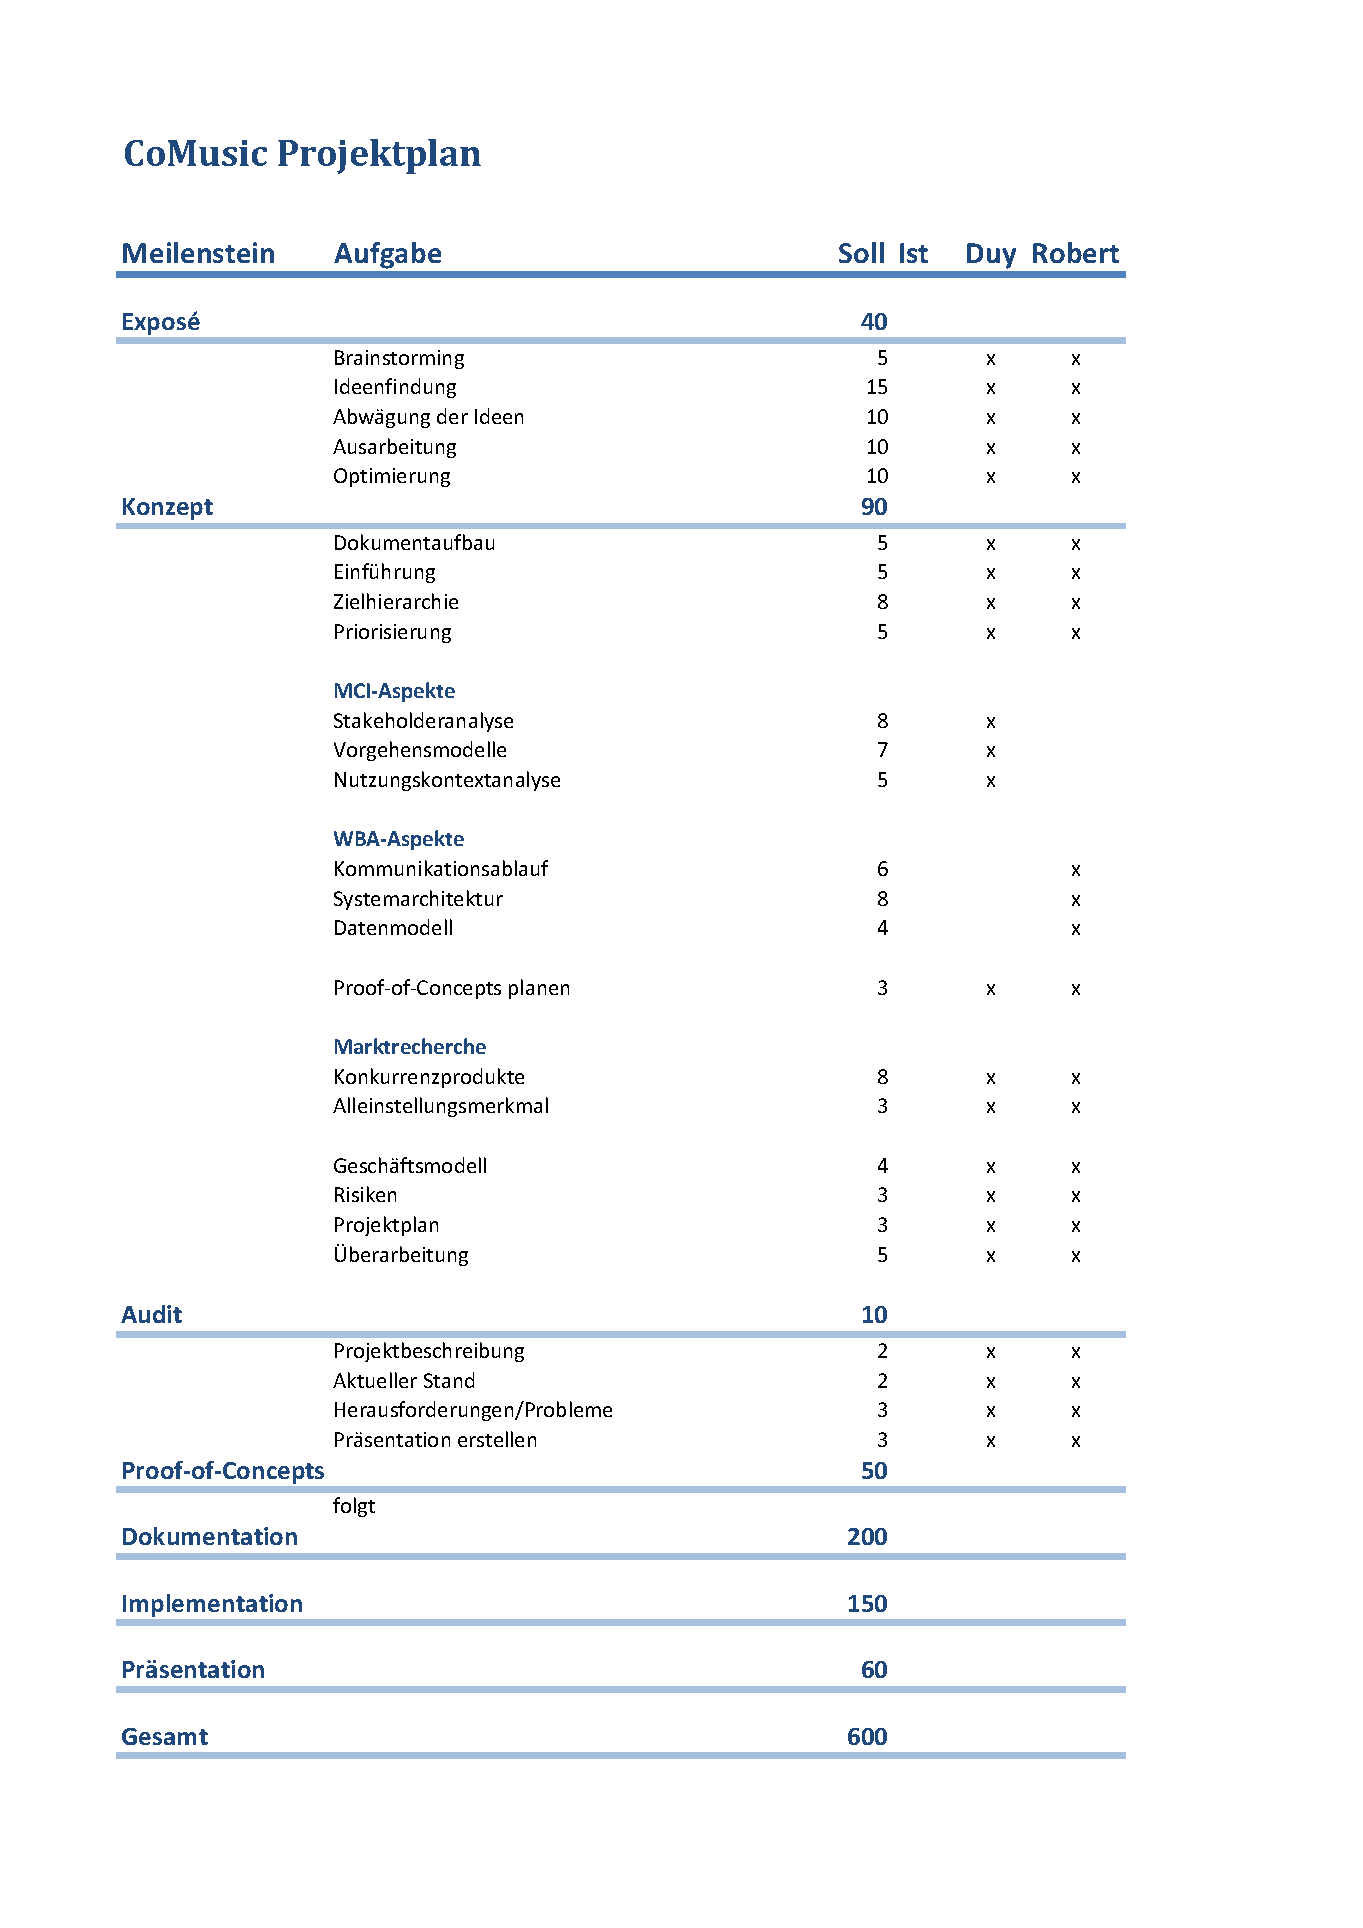
\includepdf[pages=-]{../Projektplan/EIS_Projektplan_KhuongKellermann.pdf} 

% hier aus excel einfügen

%%%%%%%%%%%%%%%%%%%%%%%%%%%%%%%%%%%%%%%%%%%%%%%%%%%%%%%%%%%%%%%%%%%%%%%%%%%%%

\newpage

\listoffigures

\newpage

\listoftables

\end{document}
